\section{Modello del sistema}
Nel paragrafo precedente ho detto che l'unica interazione possibile tra il sistema è l'esterno è l'applicazione di una forza sul carrello. Nella pratica, questo significa che è presente un motore vincolato al carrello in qualche modo. Mentre la natura del vincolo non è interessante, dobbiamo invece prestare particolare attenzione al tipo di motore utilizzato. Un motore esercita una forza che dipende sia da un segnale di controllo esterno, sia dallo stato interno dello stesso. È quindi conveniente separare lo studio del sistema in due: pendolo-carrello e motore.

\begin{figure}[thb]
    \centering
    %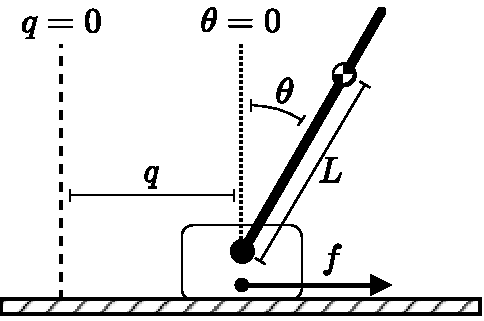
\includegraphics[width=0.4\textwidth]{assets/pic.png}
    \caption{Pic system. Qui ci va circa la stessa figura sopra, ma con l'immagine del motore collegato al carrello. }%todo
    \label{fig:pic-real}
\end{figure}

\subsection{Pendolo e carrello}
È immediato ricavare le equazioni del moto usando l'approccio Lagrangiano. Inizio fissando alcuni parametri che possono essere misurati sperimentalmente; sono riportati in tabella \ref{tab:parametri}. Posso quindi scrivere l'espressione per l'energia cinetica $T$ e potenziale $V$ del sistema:

\begin{equation*}
    \begin{aligned}
        T &= \frac 1 2 M  \dot q^2 +  \\ %todo
        V &= mgL \cos\theta
    \end{aligned}
    \hspace{20pt} \text{con } q \in \R, \theta \in ]-\pi, +\pi].
    \label{eq:energy}
\end{equation*}
La Lagrangiana $\mathcal L$ è data da:
\begin{equation*}
    \mathcal L = T - V
\end{equation*}
e posso ricavare le equazioni del moto usando le equazioni di Eulero:
\begin{equation*}
    \begin{aligned}
        asdasdasd %todo scrivi eq eulero
    \end{aligned}.
    \label{eq:moto-sistema}
\end{equation*}
%todo
Qui ci dovrei mettere due considerazioni sulle forze (in particolare sugli attriti...)
Studio inoltre i punti di equilibrio del sistema:
\begin{equation*}
    \left. \frac \partial {\partial \theta}\right |_{V=V_{eq}} V =  0 \implies V_{eq} = \{0, \pi\}.
\end{equation*}


\begin{table}[htbp]
    \centering
    \begin{tabular}{@{}ll@{}}
        \toprule
        \textbf{Correct}     & \textbf{Incorrect}         \\
        \midrule
        \( A \implies B \)   & \( A \Rightarrow B \)      \\
        \( A \impliedby B \) & \( A \Leftarrow B \)       \\
        \( A \iff B \)       & \( A \Leftrightarrow B \)  \\
        \bottomrule
    \end{tabular}
    % Tra graffe ci sta il nome che viene visualizzato nell'elenco delle tabelle
    \caption[Parametri]{Parametri}
    %todo
    \label{tab:parametri}
\end{table}
\todo{fai tabella}

\subsection{Motore}
\todo{fix reference}
\ref{https://homepages.laas.fr/lzaccari/seminars/DCmotors.pdf}
Per questa applicazione è sufficiente usare un motore DC a spazzole. Il motore è attivato applicando una differenza di potenziale $U$ tra le due armature e il verso di rotazione dipende dal segno della differenza di potenziale. Variando $U$ si ottiene grossolanamente un controllo sulla velocità di rotazione. Io voglio controllare la forza che il motore esercita sul carrello e devo quindi trovare la relazione tra differenza di potenziale e coppia $\tau$.
Fisso alcuni parametri relativi al motore, riportati in tabella \ref{tab:parametri-motore}.

\begin{table}[htbp]
    \centering
    \begin{tabular}{@{}ll@{}}
        \toprule
        \textbf{Correct}     & \textbf{Incorrect}         \\
        \midrule
        \( A \implies B \)   & \( A \Rightarrow B \)      \\
        \( A \impliedby B \) & \( A \Leftarrow B \)       \\
        \( A \iff B \)       & \( A \Leftrightarrow B \)  \\
        \bottomrule
    \end{tabular}
    % Tra graffe ci sta il nome che viene visualizzato nell'elenco delle tabelle
    \caption[Parametri motore]{Parametri motore}
    %todo
    \label{tab:parametri-motore}
\end{table}
\todo{fai tabella}


Un motore DC è regolato dalle equazioni: \todo{qui devo ritrovare il pdf che spiega tutto bene e decidere se fare io i disegni o se citare semplicemente altri paper}
\begin{equation*}
    \left\{
    \begin{aligned}
        U &= L_a \dot J + R_a J + K_e \omega \\
        \tau &= K_m J
    \end{aligned}
    \right.
    .
\end{equation*}

La coppia è proporzionale alla corrente che scorre nel motore. Si possono realizzare diversi circuiti di alimentazione che controllano direttamente la corrente ma il sistema che ho realizzato nella sezione \ref{sec:sistema-reale} può solo controllare il voltaggio. In più, il sistema non ha un sensore per misurare la corrente che passa nel motore.
Per trovare una soluzione al mio problema inizio risolvendo il sistema per $U$:
\begin{equation*}
    \begin{aligned}
        U &= L_a \partiald t \left(\frac \tau {K_m}\right) + R_a \frac \tau {K_m} + K_e \omega \\
        &= \frac {L_a} {K_m} \dot\tau + \frac{R_a}{K_m}  \tau + K_e \omega.
    \end{aligned}
\end{equation*}
In linea di principio questo è tutto quello che mi serve per controllare il motore, tuttavia, il termine che contiene $\dot \tau$ ha un coefficiente che non è facile da misurare con gli strumenti che ho a disposizione. Scelgo quindi di trascurare questo termine. Questa scelta è giustificata dal fatto che il segnale di controllo $\tau$ cambia solamente ogni $\Delta t$ secondi e posso scegliere $\Delta t$ in modo che sia maggiore del tempo del transiente dovuto a $\Delta \tau$.

Ricordando che $\tau$ e $\omega$ sono proporzionali a $f$ e $v$, trovo che questo modello dipende solo da due parametri determinabili sperimentalmente, $A$ e $B$:
\begin{equation*}
    U = A f + B v.
\end{equation*}
La determinazione di questi parametri è descritta nel paragrafo \ref{subsec:parametri-motore}.